\chapter{Algebraic Review}
\label{ch:algebra}

In this chapter, we shall discuss the algebraic theoretical background that grounds cryptography schemes.


\section{Basic structures}
% groups, quotient groups, cosets, rings, quotient rings, fields

\begin{definition}[Group]

A non-empty set G is called a group under the operation $*$, if it satisfies the following three axioms:

\begin{alineas}
    \item  (Closure) G is closed under $*$, i.e, for all $a,b\in G$, the result $a*b$ is also in $G$;
    \item (Associativity) $(a* b)* c = a\times (b*c)$, for all $a,b,c\in G$;
    \item (Existence of identity) There exists $e\in G$ such that $a*e=e*a=a$ for all $a\in G$;
    
    We shall denote the group as $(G,*)$. If, in addition to the above axioms, the group also satisfies the next property, it is called an \textbf{abelian group}.
    
    \item (Commutativity) For all $a,b\in G$, $a*b=b*a$.
\end{alineas}
\end{definition}

\begin{definition}[Subgroup]
Let $(G,\cdot)$ be a group, $H\subseteq G$ is a subgroup of $G$ if it satisfies the following:
\begin{itemize}
    \item $H\neq\varnothing$;
    \item $H$ is closed taking products: $a,b\in H\Rightarrow a\cdot b\in H$;
    \item $H$ is closed under taking inverses: $a\in H\Rightarrow a^{-1}\in H$.
\end{itemize}
Associativity is inherited by $G$ and the existence of identity element can be deduced by the above properties \cite{omn}.
\end{definition}

\begin{definition}[Ring]
    A set $R$ is called a (commutative) \textit{ring} if it has two operations: addition ($+$) and multiplication ($\times$) satisfying the following properties:

\begin{alineas}
    \item $R$ is an abelian group under addition
    \item (multiplicative associativity) $(a\times b)\times c = a\times (b\times c)$, for all $a,~b,~c\in R$ ;
    \item (distributivity) $a\times (b+c)=a\times b + a\times c$ for all $a,~b,~c\in R$;
    \item (multiplicative commutativity) $a\times b=b\times a$ for all $a,~b\in R$;
    \item (multiplicative identity) There exists an element $1$, such that, $1\times a = a\times 1 = a,$ for all $a\in R$.
\end{alineas}

Property d) is not mandatory for general non-commutative rings, but in this text, the term ``ring'' indicates a commutative one. Some examples of rings: $\mathbb{Z}$, ring of integers; $\mathbb{Z}_n$, the integers $\bmod$-$n$ and $\mathbb{Z}[X]$, set of polynomial with integer coefficients. The latter is a special ring that will be the base of our encryption schemes.
\end{definition}

\begin{definition}[Ideal]
    Given a ring $R$, a subset $I\subseteq R$ is called an \textit{ideal} of $R$ if its an additive subgroup of $R$ and satisfies:
$$r\times i \in I\text{ for all } r\in R,~i\in I$$
\end{definition}
Every ideal has a set of generators $G=\{g_1,\ldots,g_n\}$, such that 
$$I=(G)=\Big\{\sum_{i=1}^{n}g_ir_i|r_i\in R\Big\}$$
$G$ is called a \textit{basis} of $I$ if its elements are linearly independent. $I$ is a \textit{principal ideal} if $G$ has just a single element.

Two ideals $I$ and $J$ are called \textit{relatively prime ideals} of a ring $R$ if $I+J=R$, where $I+J=\{i+j|i\in I,j\in J\}$.

An example of (principal) ideal of the ring of integers is $(2)=\{2r|r\in\mathbb{Z}\}$, so-called even numbers. One can easily verify that it satisfies all the above properties.

\begin{definition}[Fields]
    A Field $F$ is a commutative ring, where for every non-zero element $a\in F$ there exists $a^{-1}\in F$ such that $aa^{-1}=1$, being $1$ the ring unity element.

    $\mathbb{Q},\mathbb{R}$ and $\C$ are examples of fields.
\end{definition}

\section{Homomorphisms and Quotient Rings}
\begin{definition}[Ring homomorphism] Let $R$ and $S$ be rings. A map $\varphi:R\to S$ is called a ring homomorphism if it preserves addition/multiplication operations and the unity element:
\begin{align*}
    \varphi(a+b)&=\varphi(a)+\varphi(b)\\
    \varphi(a\times b)&=\varphi(a)\times \varphi(b)\\
    \varphi(1_R)&=1_S
\end{align*}
Similarly, we can define group homomorphisms that will preserve their unique underlying operation.
\end{definition}
Some ring homomorphisms examples:
\begin{alineas}
    \item Integer modular reduction operation:
\begin{align*}
    \varphi&:\Z\to\Z_n\\
    \varphi(a)&=a(\bmod~n)
\end{align*}

\item Polynomial evaluation at $a\in R$:
\begin{align*}
    \varphi_a&:R[X]\to R\\
    \varphi_a(p(X))&=p(a),
\end{align*} where $R[X]$ is the set of polynomials with coefficients in a ring $R$
\end{alineas}

\begin{definition}[Isomorphism]
    A map $\varphi:R\to S$ is called an isomorphism if it is a bijective homomorphism. In this case, we denote $R\cong S$
\end{definition}

\begin{definition}[Cosets]
    
\end{definition}
\section{Cyclotomic polynomials}

In this section, we define and review some properties of cyclotomic polynomials, which will play a central role in the homomorphic cryptography setup.

\begin{definition}[Roots of unity] The $n^{th}$ roots of unity are the solution set of the equation $x^n-1=0$ in the field of complex number $\mathbb C$:
$$\sqrt[n]1=\{\zeta_n^k;k=0,1,\ldots,n-1\},$$
where\footnote{In Euler's notation $\exp{(i\theta)}=\cos\theta+i\cdot\sin\theta$} $\zeta_n=\exp{(2\pi i/n)}$
\end{definition}
In the complex plane, these roots are distributed over the unitary circumference and equally separated by an angle of $2\pi/n$. Figure \ref{fig:roots_of_unity} show the example of the $8^{th}$ roots of unity.

\begin{figure}[!htb]
    \centering
    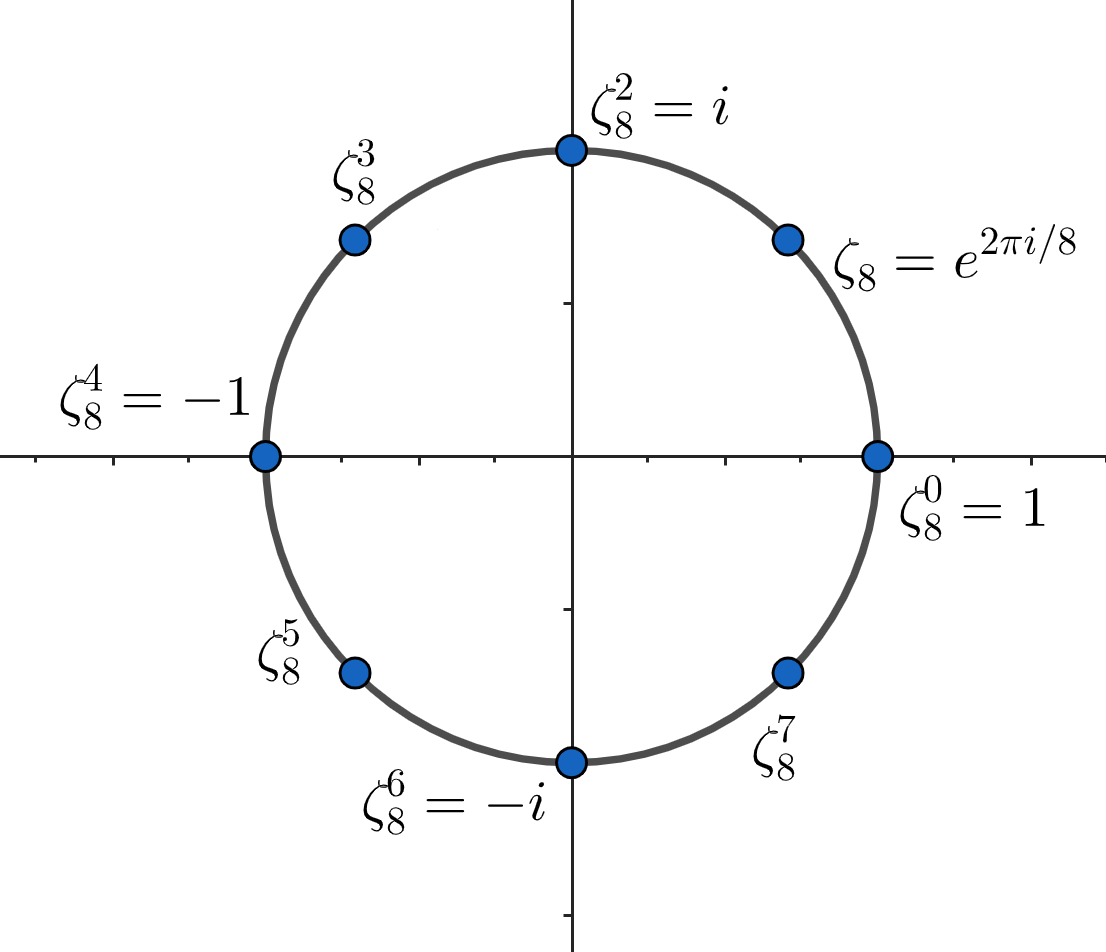
\includegraphics[scale=0.4]{files/figures/roots_of_unity.png}
    \caption{$8^{th}$ roots of unity}
    \label{fig:roots_of_unity}
\end{figure}

\begin{definition}[Primitive roots of unity]\cite{brilliant}\label{def:prim_roots}
The $n^{th}$ primitive roots of unity are:
$$\{\zeta \in \mathbb C;\zeta^n=1\text{ and }\zeta^k\neq1,\forall ~ k<n \},$$
for positive integers $k$. They are the subset of $n^{th}$ roots of unity which are not $k^{th}$ roots of unity, for all $k<n$. They can be alternatively defined as:
$$\{\zeta_n^k;1\leq k \leq n,\gcd(k,n)=1\}$$
\end{definition}
From the Figure \ref{fig:roots_of_unity} example, the $8^{th}$ primitive roots of unity are $\zeta_8,\zeta_8^3,\zeta_8^5,\zeta_8^7$.
% Indeed, $\zeta_n^k=\exp(2k\pi i/n)$ will be equal to $1$ if, and only if the exponent is an integer multiple of $2\pi i$, which is not the case when $\gcd(k,n)=1$, since $k/n$
% tmp\cite{brilliant}

\begin{definition}[Cyclotomic polynomial] \label{def:cyclo}The \textit{$n$-th cyclotomical polynomial} is defined as:
\begin{align*}
    \Phi_n(x) = \prod_{\substack{1\leq k \leq n\\ \gcd(k,n)=1}}^{n}(x-\zeta_n^k)
\end{align*}
\end{definition}

Notice that its roots are the $n^{th}$ primitive roots of unity.

Using the definition, we can derive some cyclotomical polynomials, for example $\Phi_1(x)=x-1$ trivially, and $\Phi_2(x)=x+1$, since from the $2^{nd}$ roots of unity $-1$ and $+1$, only $-1$ are primitive ones.

The $3^{rd}$ primitive roots of are $\zeta_3^1$ and $\zeta_3^2=\overline{\zeta_3^1}$, then:
\begin{align}
    \Phi_3(x)&=(x-\zeta_3^1)(x-\zeta_3^2)\nonumber\\
    &=x^2-x(\zeta_3^1+\zeta_3^2)+\zeta_3^1\zeta_3^2\nonumber\\
    &=x^2-x(\zeta_3^1+\overline{\zeta_3^1})+e^{2\pi i(1+2)/3}\label{eq:zeta3}\nonumber\\
    &=x^2-x(2\cdot\cos(2\pi/3))+e^{2\pi i}\\
    &=x^2+x\left(2\cdot \frac12\right)+1\nonumber\\
    &=x^2+x+1\nonumber
\end{align}

The equality (1) holds due to the sum of complex conjugates being equal to two times the real part since we cancel out the imaginary terms.

\begin{theorem} \label{teoremaco}For all positive integers $n$ we have:
$$\displaystyle x^n-1=\prod_{d|n}\Phi_d(x)$$
\end{theorem}

The above theorem provides a analytical formula to recursively generate the cyclotomic polynomials:
$$\displaystyle\Phi_n(x)=\dfrac{x^n-1}{\displaystyle\prod_{\substack{d|n\\d\neq n}}\Phi_d(x)}$$

We can use it to derive simpler, and non-recursive expressions for particular interesting cases:

\begin{corollary}[Prime Cyclotomical Polynomial]
If $p$ is a prime number, then:
$$\Phi_p(x)=x^{p-1}+x^{p-2}+\ldots+x+1$$
\end{corollary}

\begin{proof}
By the previous theorem, and the fact that the only $d<p$ satisfying $d|n$ is $d=1$:

$$\Phi_p(x)=\dfrac{x^p-1}{\displaystyle\prod_{\substack{d|p\\d\neq p}}\Phi_d(x)}=\dfrac{x^p-1}{\Phi_1(x)}=\dfrac{x^p-1}{x-1}$$

The polynomial division algorithm concludes that such a division actually results in what is claimed in the corollary.

An easy way to assert it, is by multiplying the divisor $x-1$ by $\displaystyle\sum_{i=0}^{p-1}x^i$ and checking if it is equal to $x^p-1$:
\begin{align*}
    (x-1)\left(\sum_{i=0}^{p-1}x^i\right)&=\sum_{i=0}^{p-1}x^{i+1}-\sum_{i=0}^{p-1}x^i\\
    &=\sum_{i=0}^{p-1}x^{i+1}-x^{i}\\
    &=x^{(p-1)+1}-x^{0}\\
    &=x^{p}-1
\end{align*}
\end{proof}
The following formula will be crucial to instantiate plaintext and ciphertext spaces in the encryption schemes.
\begin{corollary}[Power of Two Cyclotomic Polynomial]
If $M=2^n$, for a given positive integer $n$, then:
$$\Phi_M(x)=x^{M/2}+1$$
\end{corollary}
\begin{proof}
We'll proceed by strong induction in $n$ \cite{herstein1996abstract},  proving an equivalent statement\footnote{One can easily verify that $\dfrac{x^{M}-1}{x^{M/2}-1} = x^{M/2}+1$ using the polynomial division algorithm for example, or multiplying the divisor with the quotient}: 
\begin{equation}
\label{eq:phim}
    \Phi_{M_n}(x) = \dfrac{x^{M_n}-1}{x^{M_n/2}-1}
\end{equation}
We're denoting $2^n$ by $M_n$ to have a cleaner notation of nested exponents; hence $M_n/2=M_{n-1}$.

(Base case) For $n=1$, $\Phi_{M_1}(x)=\Phi(2)=x+1$, as we derived before. This is the LHS of \ref{eq:phim}. The RHS is $\frac{x^2-1}{x-1}=\frac{(x+1)(x-1)}{x-1}=x+1$, so the formula is valid in this case.

(Inductive Hypothesis) Assume that \ref{eq:phim} hold for $M_k$ for all $k<n$ positive integers.

(Inductive Step) Let's deduce that it also holds for $M_n$: By Theorem  \ref{teoremaco}, we have:
\begin{align*}
    \Phi_{M_n}(x) &= \dfrac{x^{M_n}-1}{\displaystyle\prod_{\substack{d|M_n\\d\neq M_n}}\Phi_d(x)}
\end{align*}
Notice that $\{d\in\mathbb{Z}^+;d|M_n\} = \{M_0,M_1,\ldots,M_{n-1}\}$, i.e., the divisors of $M_n$ are the powers of two with exponent less than $n$. Then our expression becomes:
$$\Phi_n(x) = \dfrac{x^{M_n}-1}{\Phi_{M_0}\Phi_{M_1}\ldots\Phi_{M_{n-1}}}$$
Using $\Phi_{M_0}(x)=x-1$ and the inductive hypothesis, we can rewrite the denominator as:
\begin{align*}\Phi_{M_0}\Phi_{M_1}\ldots\Phi_{M_{n-1}}&=(x-1)\cdot \dfrac{x^{M_1}-1}{x^{M_0}-1}\cdot\dfrac{x^{M_2}-1}{x^{M_{1}}-1}\ldots\cdot\dfrac{x^{M_{n-1}}-1}{x^{M_{n-2}}-1}\\&=x^{M_{n-1}}-1,\end{align*}
since that's the only term left after canceling out left numerators with right denominators. We then conclude:
\begin{align*}
    \Phi_{M_n}(x) &= \dfrac{x^{M_n}-1}{x^{M_{n-1}}-1}=x^{M_n/2}+1
\end{align*}
\end{proof}

Another interesting property of cyclotomic polynomials, which is quite impressive, is the following theorem:
\begin{theorem}
``For any positive integer $n$ we have $\Phi_n(x)\in\Z[x]$, That is, $\Phi_n(x)$ is a polynomial
with integer coefficients.''\cite{sun2013cyclotomic}
\end{theorem}
We defined these polynomials as products of a bunch of complex numbers, but the coefficients end up in the integers! Such a beautiful property will allow us to determine later quotient rings like $\Z[x]/(\Phi_n(x))$ to our encryption context.

\section{Lattices}

This section introduces lattices and hard lattice problems that will base the security of fully homomorphic schemes.
\begin{definition}[Lattice]
Let $b_1,\ldots,b_k\in\mathbb{R}^n$ be linearly independent vectors, then
$$\mathcal{L}=\Big\{\sum_{i=1}^ky_ib_i\left|\right.y_i\in\mathbb{Z}\Big\}$$
is a ($n$-dimensional) \textbf{lattice} and $(b_1,\ldots,b_k)$ its \textbf{basis}. If we create a $n\times k$ matrix $\mathbf B$, where the $i$-th column is $b_i$, then we can write
$$\mathcal{L}(\mathbf B)=\{\mathbf B y| ~y\in \mathbb{Z}^k\}\subset \operatorname{span}(B)$$
\end{definition}
Figure \ref{fig:lattices} shows two geometrical examples in $\R^2$, the first one using canonical basis $(e_1,e_2)$, and the second suing $B=(b_1,b_2)$, with $b_1=e_1$ and $b_2=\frac{1}{\sqrt2}(2,1)$
\begin{figure}[!htb]
\centering
\begin{subfigure}{.5\textwidth}
  \centering
  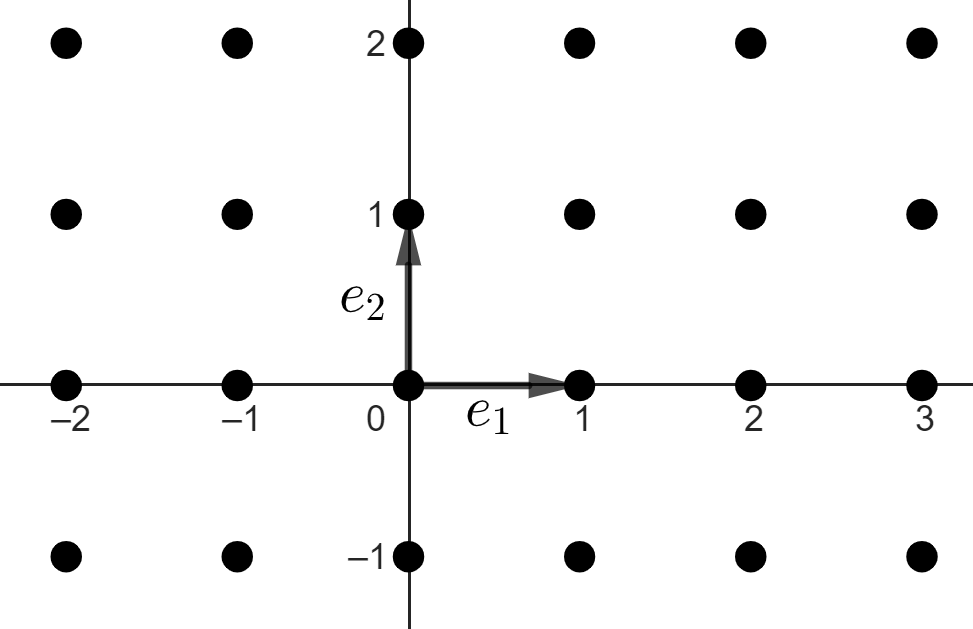
\includegraphics[scale=0.25]{files/figures/lattice_canonical.png}
  \caption{Canonical basis}
  \label{fig:canonical_lattice}
\end{subfigure}%
\begin{subfigure}{.5\textwidth}
  \centering
  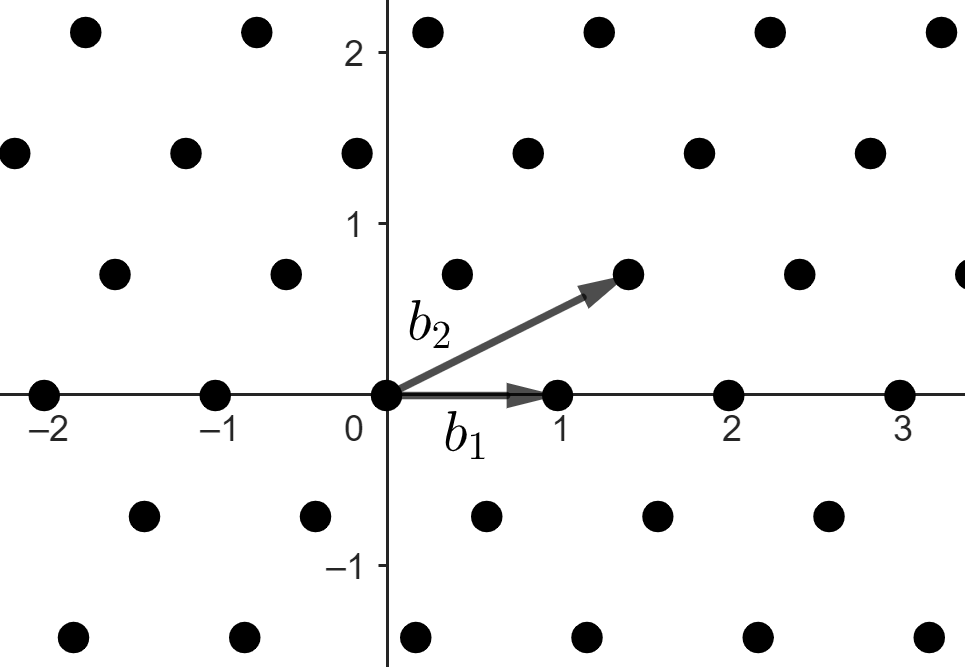
\includegraphics[scale=0.25]{files/figures/lattice2.png}
  \caption{Basis $B=(b_1,b_2)$}
  \label{fig:sub2}
\end{subfigure}
\caption{Lattices examples}
\label{fig:lattices}
\end{figure}

\begin{definition}[Ideal lattice]
An \textbf{ideal lattice} $\mathcal L$ is a lattice that is closed under addition and multiplication: For $v_1,v_2\in \mathcal{L}$, we have $v_1+v_2\in \mathcal{L}$ and $v_1\cdot v_2\in\mathcal L$, with the operations inherited by $\R^n$
\end{definition} 

\begin{definition}[Successive minima]
The $i^{th}$ successive minima of an $n$-dimensional lattice $\mathcal L$, denoted by $\lambda_i(\mathcal L)$ is the smallest $r$ such that origin-centered ball with radius $r$ contains $i$ linearly independent (LI) lattice vectors.
\end{definition}

In Figure \ref{fig:canonical_lattice} example $\lambda_1(\mathcal L)=\lambda_2(\mathcal L)=1$, since the unity ball contains the two LI canonical vectors. But in Figure \ref{fig:sub2}, it's not so obvious, but $\lambda_1(\mathcal L)=||b_3||_2\approx 0.82$, where $b_3=b_2-b_1$ and $\lambda_2(\mathcal L) = ||b_4||_2\approx0.92$, with $b_4=b_3-b_1$. In Figure \ref{fig:successive_minimas}, we can visually verify that $b_3$ and $b_4$ are indeed LI.

\begin{figure}[!htb]
\centering
\begin{subfigure}{.5\textwidth}
  \centering
  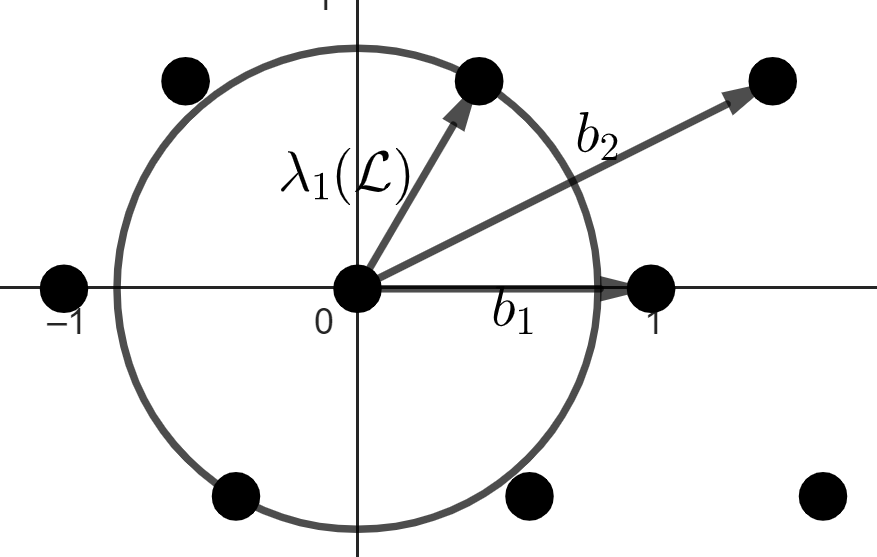
\includegraphics[scale=0.25]{files/figures/lambda1.png}
  \caption{$1^{st}$ successive minima}
  \label{fig:lambda1}
\end{subfigure}%
\begin{subfigure}{.5\textwidth}
  \centering
  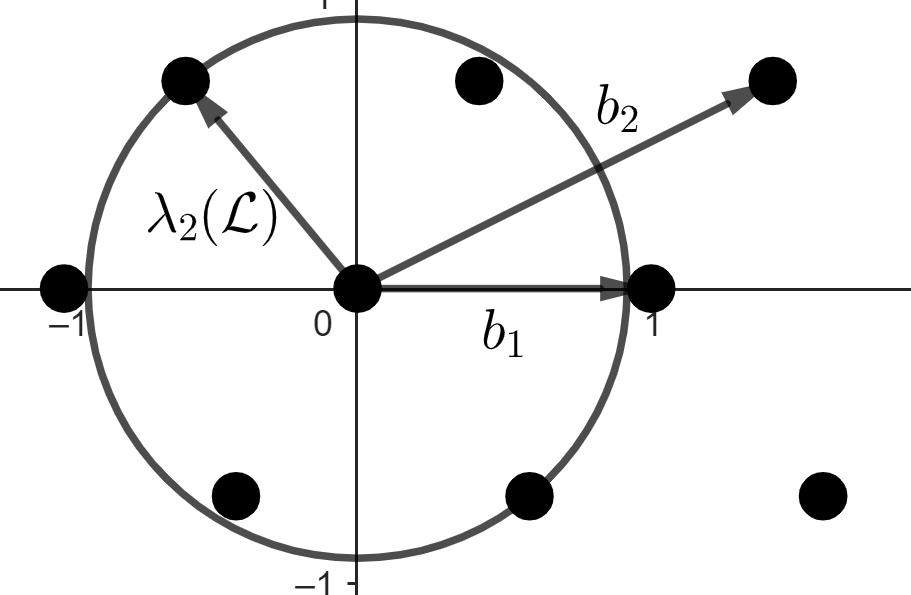
\includegraphics[scale=0.23]{files/figures/lambda2.png}
  \caption{$2^{nd}$ successive minima}
  \label{fig:lambda2}
\end{subfigure}
\caption{Successive Minimas}
\label{fig:successive_minimas}
\end{figure}

\subsection{Lattice Problems}
Now we can define two famous lattice problems, all of them considered NP-hard \cite{hardnes}. ``The approximation factor $\gamma$ is usually taken as a function of lattice dimension $\gamma(n)$.'' \cite{ppt_dm}

\begin{definition}[Shortest Vector Problem - SVP]\label{def:svp} Given a lattice $\mathcal L$ and a norm $||.||$, find a non-zero $v\in\mathcal L$ such that $||v||\leq\gamma \lambda_1(\mathcal L)$, i.e., the non-zero lattice vector closest to the origin. 
\end{definition}

In the above example of $\mathcal L (b_1,b_2)$ the shortest vector is $b_3$, for $\gamma=1$.

\begin{definition}[Shortest Independent Vector Problem - SIVP] Given a lattice $\mathcal L$ of dimension $n$ and a norm $||.||$, find $n$ linearly independent vectors $v_1,v_2,\ldots,v_n$ such that $\displaystyle\max_{i}{||v_i||}\leq\gamma\lambda_n(\mathcal L)$.
\end{definition}

For $\mathcal L (b_1,b_2)$, the solution for the $\text{SIVP}_\gamma$ with $\gamma=1$ is $\{b_3,b_4\}$.

These problems establish the so-called \textit{lattice-based cryptography}, which are cryptosystems that have their security based on solving the above problems of variants. All The fully homomorphic encryption schemes we shall dive deeper into in the next chapter are lattice-based.

\subsection{Ring Learning with Errors}
Now that we have computationally complex challenges, the next step is, based on these results, constructing a concrete secure cryptography scheme. The following two problems are a step in this direction.

\begin{definition}[Learning with Errors - LWE] Given an integer $n$, a prime integer $q$ such that\footnote{$\poly(n)$ denotes a polynomial function of $n$.} $2\leq q\leq \poly(n)$ and a distribution $\chi$ over $\Z_q$. Fix $\bds\in \Z_q^n$, the Search $\operatorname{LWE}_{n,q,\chi}$ problem is to recover $\boldsymbol s$, given observations $(\bda_i,b_i)$, where\footnote{Notation $x\xlongleftarrow[]{\chi}S$, means $x$ were drawn from distribution $\chi$ over the set $S$, and $\mathcal{U}$ is the uniform distribution}:
\begin{align*}
    \bda_i&\xlongleftarrow[]{\mathcal U}\Z_q^n\\
    b_i &= \langle \bda_i,\bds\rangle + e_i~(\bmod q)\\
    e_i&\xlongleftarrow[]{\chi}\Z_q
\end{align*}
The Decision $\operatorname{LWE}_{n,q,\chi}$ is the problem of distinguishing between the distribution of $(\bda_i,b_i)$ gotten from the above procedure and the uniform distribution over $\Z_q^{n+1}$.
\end{definition}
Under reasonable assumptions on $\chi$, if an algorithm efficiently solves the above (decision) problem, GapSVP and SIVP can also be solved efficiently \cite{regev09}. 

LWE provides a nice setup for private key encryption since one can expose $(\bda_i,b_i)$ while the hardness of lattice-based problems guarantees the security of $\bds$. Further, we shall name $(\bda_i,b_i)$ as the public key and $\bds$ as the private key. One can still prove that Seach-LWE can be reduced to Decision-LWE \cite{lyubashevsky10}, which completes the cycle.

In our main FHE construction, the scheme is based on a variant of LWE:

\begin{definition}\label{def:rlwe}
[Ring Learning with Errors - RLWE] Set integers $n,q$, with $n$ being a power of two, and $2\leq q \leq \poly(n)$. Let $f(x)=x^n+1$ (the $2n$-th cyclotomic polynomial), define $\mathcal R=\Z[X]/( f(X))$, a distribution $\chi$ over $\mathcal R$ and $\mathcal{R}_q=\mathcal R/(q) =\Z_q[X]/(f(X))$ which can be represented by polynomials with integer coefficients wrapped by $q$ and with degree up to $n-1$.

Let $s=s(x)\in \mathcal{R}_q$ be an element chosen uniformly from the ring. The Search $\operatorname{RLWE}_{n,q,\chi}$ problem is to recover $s$ given a set of pairs $(a_i,b_i)\in \mathcal{R}_q^2$, with
\begin{align*}
    a_i&\xlongleftarrow[]{\mathcal U}\mathcal{R}_q\\
    b_i &= a_i\cdot s + e_i~(\bmod q)\\
    e_i&\xlongleftarrow[]{\chi}\mathcal R
\end{align*}
Analogously with LWE, we define Decision $\operatorname{RLWE}_{n,q,\chi}$ as the problem of distinguishing the distribution of the above pairs from a uniform distribution over $\mathcal{R}_q^2$. 
\end{definition}
% An observation in both LWE and RLWE is that, in practice, the distribution $\chi$ of $e_i$ must yield small enough errors compared to $q$. That's why we omit $\bmod q$ after the equation of $b_i$'s. Such a thing would guarantee that $b_i$ is an element of $\Z_q$ or $\mathcal{R}_q$.
The Search RLWE can also be reduced to Decision RLWE. Moreover, under some assumptions over the parameters $n,q,\chi$, which we won't state here, an efficient algorithm for Decision $\operatorname{RLWE}_{n,q,\chi}$ implies an efficient algorithm for solving SVP \cite{lyubashevsky10}.

The choice of $f(x)$ being a power of two cyclotomic polynomial is purely technical; in general, $f(x)$ could be any cyclotomic polynomial, and all the theory would still holds. We shall further want to multiply two instances of the cyclotomic ring, and there is a method based on Fast Fourier Transform to perform such task \cite{fftmult}. But choosing specifically $f(x)=x^n+1$ admits optimized and faster implementations \cite{swifft}.


\chapter{Fully Homomorphic Encryption}
This chapter gives an overview of the FHE research. Section \ref{sec:privhom} returns in 1978 and revises the original proposal of the existence of FHE schemes \cite{Rivest1978}, which was called \textit{privacy homomorphisms}. Section \ref{sec:gentry} explores Gentry's solution through his Ph.D. thesis \cite{gentry2009fully} proving such existence. Section \ref{sec:ckks} presents the so-called CKKS scheme \cite{ckks17}, a practical and modern scheme that allows approximate encryption of complex (so, also real) numbers, well suitable for machine learning applications. 

\section{Privacy Homomorphisms}
\label{sec:privhom}
Assume we can represent the unencrypted data by an algebraic structure $\mathcal P= (S;f_1,\ldots,f_k)$, i.e., a set $S$ ported with the operations $f_1,\ldots,f_k$. We will further call this structure the plaintext space.

An alternative algebraic structure, the ciphertext space $\cipher=(S',f'_1,\ldots,f'_k)$, is constructed to represent the encrypted data. To build a \textit{privacy homomorphism} \cite{Rivest1978},  one needs a decryption function $\phi:S'\to S$ and its inverse $\phi^{-1}:S\to S'$ satisfying the homomorphic property from $\cipher$ do $\Plain$:
\begin{align}
    \label{privhom}
    f'_i(a,b,\ldots)&=c\Rightarrow\nonumber\\ f_i(\phi(a),\phi(b),\ldots)&=\phi(c),\text{ for } i=1,\ldots,k\\
    \text{with }a,b,&\ldots\in S'\nonumber
\end{align}
This means that for all available operations $f'_i$, its evaluation on encrypted elements must result in a value that, after decryption, corresponds to the same computation on the unencrypted domain.

An example of privacy homomorphism is the RSA cryptosystem \cite{rsa}, which uses $\Plain = (\Z_p;\times_p)$, the integers modulo $p$ with $p$ prime, and the multiplication modulo $p$. Setting $N=pq$, where $q$ is a large prime and choosing $e$ coprime with $(p-1)(q-1)$,  the ciphertext space as $(\Z_N;\times_N)$ and is connected with $\Plain$ through the encryption function:
\begin{align*}
    \phi^{-1}&:\Z_p\to\Z_N\\
    \phi^{-1}(x)&=x^e(\bmod N)
\end{align*}
Taking $x,y\in\Z_p$ and its encrypted versions $x'=\phi^{-1}(x),~y'=\phi^{-1}(y)$, we have:
\begin{align*}
    x'\times_N y'&= (x^e)(y^e)(\bmod N)\\
    &=(xy)^e(\bmod N),
\end{align*}
which is an encryption of $xy$. Then the multiplication satisfies property \ref{privhom}, showing that such a system is indeed a privacy homomorphism.

\subsection{Requirements and Limitations}\label{subsec:reqs}
The following properties for $\cipher,\phi$ and $\phi^{-1}$ are required by the authors:
\begin{alineas}
    \item for a given element $s\in S$, its encrypted version $\phi^{-1}(s)$ should not require much more storage space;
    \item $\phi$ and $\phi^{-1}$ should be easy to compute;
    \item the operations $f_i'$ should be efficiently computable in $\cipher$;
    \item $\phi$ should not be vulnerable to the chosen plaintext attack;
    \item The operations of $\cipher$ should not be sufficient to yield an efficient computation of $\phi$.
\end{alineas}

The last requirement forces a critical restriction on such morphisms: a comparison operator ``$\leq$'' can't be available in the ciphertext space, otherwise, no secure privacy homomorphism exists.

Take for example $\Plain = (\N;+,\leq)$ and $\cipher = (W;+',\leq')$ for some $W$. A malicious party who has $\phi^{-1}(n)$ and wants to discover what $n\in\N$ generated such ciphertext can apply the following binary search strategy:
\begin{alineas}
\item compute $1'=\phi^{-1}(1)$;
\item compute $2'=1'+'1'$, then $4'=2'+'2'$;
\item continue until finding $k$, such that $\phi^{-1}(n)\leq'(2^k)'=\phi^{-1}(2^k)$
\item knowing that $n\in[2^{k-1},2^{k}]$, compute an encryption of the interval midpoint $\phi^{-1}(m)=\phi^{-1}(2^{k-1}-2^{k-2})$;
\item homomorphically compare $\phi^{-1}(n)\leq'\phi^{-1}(2^{k-1})+'\phi^{-1}(m)$;
\item repeat the last two steps properly redefining the interval until getting $n$ exactly.
\end{alineas}
This is an efficient $O(\log n)$ algorithm to compute the decryption function $\phi$, using the operations in $\cipher$ and the ability to generate encryptions of arbitrary constants (such as $1$ and $m$ in the above example).

The article finishes with the authors pondering if such an approach with all required security restrictions could be worthwhile in practice and what algebraic structures $\Plain$ would provide useful privacy homomorphisms.
% \section{First Generation Fully Homomorphic schemes}
% \begin{alineas}
% \item somewhat/fully homomorphic
% \item bootstrapping
% \item integer scheme
% \item caveats and implementation paper
% \end{alineas}

\section{Bootstrappable encryption}
\label{sec:gentry}
The existence of (useful) privacy homomorphisms remained an open problem for more than 30 years until \cite{gentry2009fully} came up with a beautiful solution in his Ph.D. thesis. He introduced a privacy homomorphism based on ideal lattices and proposed a method named bootstrapping, his most significant insight, to control ciphertext noise growth. A second paper was proposed, with a slightly simpler scheme using integers instead of lattices \cite{fhe_integers}.

This section summarizes Gentry's achievement, \ref{sub:over} with a complete summarized overview of the solution,  \ref{sub:over} describing the scheme over the integer.
% , and \ref{sub:practical} commenting about practical considerations. 
We let the explanation of the original cryptosystem over ideal lattices to Appendix \ref{appendixA} since not reading doesn't interfere in the text flow.

\subsection{Overview and Bootstrapping}
\label{sub:over}
Let's denote $\phi^{-1}(.)$ by $\enc(\pk,.)$, now requiring a public key $\pk$, and $\phi(.)$ by $\dec(\sk,.)$, where $\sk$ is a secret key. The construction also requires an evaluate algorithm $\eval(\pk;.)$ that computes a function $f$ in the ciphertext space. In the previous section's construction, this algorithm $\eval(\pk,f_i,\ldots)=f'_i(\ldots)$, i.e., the computation of $f$ in the encrypted domain won't be a direct evaluation, but a modified one, adapting to restrictions and patterns of the new space.

Take a function $f\in\mathcal P$ in the plaintext space, and some elements $s_1,s_2,\ldots\in S$, and its encrypted versions $c_i=\enc(\pk,s_i)$. Rewriting \ref{privhom} in this new notation, we get the correctness property for $f$:
\begin{align}
\label{eq:correctness}
    \dec(\sk,\eval(\pk,f,c_1,c_2,\ldots))=f(s_1,s_2,\ldots)
\end{align}
The encryption function \textbf{must add random noise to the plaintext} messages to resist the chosen ciphertext attack as required in the property (d) of \ref{subsec:reqs}. Calling $\enc(\pk,s)$ multiple times would yield different ciphertexts each time, but decrypting all of them, returns to $s$.

\begin{definition}[Fully Homomorphic Encryption - FHE]
The first definition of FHE scheme defines it as a scheme that allows anyone to evaluate ``any desired function $f$'' over the encrypted data $c_1,c_2,\ldots$ without decrypting it, just as privacy homomorphisms. \cite{gentry2009fully}
\end{definition}
In practice, what is proven is the existence of a scheme that can evaluate addition and multiplication functions, which are enough to compose any boolean circuit.
\begin{align*}
    \dec(\sk,\eval(\pk,+,c_1,c_2))=s_1+s_2\\
    \dec(\sk,\eval(\pk,\times,c_1,c_2))=s_1\times s_2\\
\end{align*}
Because of the noise added in the encryption step, if we perform multiple additions and multiplications, the noise can grow at levels that might affect the above correctness property (this will soon become clearer). Then, we introduce the following concept:
\begin{definition}[Somewhat Homomorphic Encryption - SHE] Let $F$ be a circuit of composition of additions and multiplications with a given depth. A SHE scheme satisfies the following:
$$\dec(\sk,\eval(\pk,F,c_1,c_2,\ldots))=f(s_1,s_2,\ldots)
$$
only if the depth of $F$ is less than the scheme's maximum allowed depth.
\end{definition}

The bottleneck to achieving an FHE scheme is the introduction of noise in the encryption function. A circuit $F$ with a big enough number of multiplications, for example, might not satisfy the correctness property because of the noise's size compared to the original message.

Then a process called \textit{bootstrap} (or recrypt) is introduced \cite{gentry2009fully}, which is a way of reducing the ciphertext noise by homomorphically evaluating the own scheme decryption function, producing a new ciphertext that encrypts the same message with less noise. 

To achieve a fully homomorphic scheme out of a somewhat homomorphic one, it's enough to prove that the scheme is ``bootstrappable'', i.e., that it can correctly evaluate circuits that are deeper than its own decryption circuit. 

Suppose $c$ encrypts $s$ under $\pk_1$, and we want to reduce its noise; one way to do that is to decrypt $c$ using the secret key, getting back to the plaintext space (without any noise) and then encrypt $s$ again generating a fresh and new encryption. To maintain security and not reveal the actual message, the process is done homomorphically. 

Suppose we have $\sk^* = \operatorname{Encrypt}(\sk_1,\pk_2)$, an encryption of the secret key under a second public key $\pk_2$. Define the $\operatorname{Recrypt}$ algorithm as:
\begin{align*}
   \operatorname{Recrypt}(\pk_2,\sk^*,\dec,c)&\\
   \text{Set }c^*&=\enc(c,\pk_2)\\
   \text{Output }c_2&=\eval(\pk_2,\dec,\sk^*,c^*)
\end{align*}
% The output of Recrypt is encryption of $\dec(\sk_1,c)=s$ under $pk_2$.
Figure \ref{fig:bootstrapping} illustrates this procedure through the blue arrows.

The $\enc$ function might introduce some noise to $c_2$, but as long as this noise is less than the one associated with $c$, we succeed in refreshing ciphertext noise. 

% https://q.uiver.app/?q=WzAsNCxbMCwyLCJjIl0sWzAsMCwiY14qIl0sWzMsMiwibSJdLFszLDAsImNfMiJdLFswLDEsIlxcb3BlcmF0b3JuYW1le0VuY30oXFxvcGVyYXRvcm5hbWV7cGt9XzIsXFxjZG90KSIsMCx7InN0eWxlIjp7ImJvZHkiOnsibmFtZSI6ImRhc2hlZCJ9fX1dLFswLDIsIlxcb3BlcmF0b3JuYW1le0RlY30oXFxvcGVyYXRvcm5hbWV7c2t9LFxcY2RvdCkiLDJdLFsxLDMsIlxcb3BlcmF0b3JuYW1le0V2YWx9KFxcb3BlcmF0b3JuYW1le3BrfV8yLFxcb3BlcmF0b3JuYW1le0RlY30sXFxvcGVyYXRvcm5hbWV7c2t9XiosXFxjZG90KSIsMCx7InN0eWxlIjp7ImJvZHkiOnsibmFtZSI6ImRhc2hlZCJ9fX1dLFszLDIsIlxcb3BlcmF0b3JuYW1le0RlY30oXFxvcGVyYXRvcm5hbWV7c2t9LFxcY2RvdCkiXV0=
\begin{figure}[!htb]
    \centering
    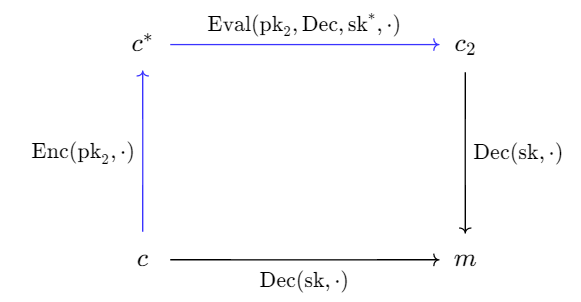
\includegraphics[scale=0.9]{files/figures/bootstrapping.png}
    \caption{Bootstrapping procedure}
    \label{fig:bootstrapping}
\end{figure}

The SHE schemes proposed by Gentry were not originally bootstrappable because the decryption was too deep. The work then dedicates a lot of effort to minimize the depth of the decryption circuit, but the ability to bootstrap is only achieved by a technique called \textit{squashing}, where the encrypter starts the decryption process, giving partial hints to the decryptor. Although he could arrive at an FHE scheme, squashing introduced additional security requirements.

\subsection{An integer scheme}
\label{sub:int}
A second work from Gentry \cite{fhe_integers} introduces a conceptually simpler SHE scheme using the ring of integers as the underlying algebraic structure instead of ideal lattices. 

We start with a private key scheme and then transform it into a public key one:

\begin{itemize}
    \item $\operatorname{KeyGen}$ - sets the private key as an odd integer $p$
    \item $\enc(p,m)$ - given a bit message $m\in\{0,1\}$, outputs $c=pq+2r+m$, where $q$ and $r$ are choosen randomly in some prescribed interval.
    \item $\dec(p,c)$ - outputs $(c\bmod p)\bmod 2$
\end{itemize}

Correctness property can be easily checked, assuming $2r<p/2$:
\begin{align*}
    &\dec(p,\enc(p,m))\\
    &=\dec(p,pq+2r+m)\\
    &=((pq+2r+m)\bmod p)\bmod 2\\
    &=(2r+m)\bmod 2\\
    &=m
\end{align*}

Let's emphasize the need for bootstrapping with a toy example.

Let's say we want to add $m=1$ continuously. Set $p=29$, and let's suppose the encryption algorithm sampled $q=8, r=3$. Now, take the ciphertext $pq+2r+m$ and add-t to itself $c+c = p(2q)+4r+m+m$.

In the decryption function, the modulo-p reduction will eliminate $p(2q)$, and mod 2 will output us $m+m = 0$ as desired.

In general, if $\alpha\geq 1$ is an integer., $\alpha c=p(\alpha q)+2\alpha r+\alpha m,$

If we want to discover how many times we can add $c$ to itself and the decryption still works, the only condition is $2\alpha r<p$. Solving the inequality for $p=29,r=3$ we get $\alpha<29/6\approx 4.83$. So for $\alpha = 5$ we have no guarantee that the scheme will work.

Since $\alpha = 5$ is odd $\alpha m = 1$, so we would like $\dec(29,5c)=1$, but:
\begin{align*}
    &~~~\dec(29,5c)\\
    &=\dec(29,29\cdot(5 q)+2\cdot5 r+5 m)\\
    & = ((29\cdot(5 q)+30+5 m)\bmod 29)\bmod 2\\
    &=(1+5m)\bmod2\\
    & = 6\bmod 2\\
    & = 0
\end{align*}

Then decryption failed because the error was sum up to $5\alpha r$ and eventually got bigger than $p$.

To obtain a public key encryption scheme out of the above private key one, we set:

$\pk = (x_1,\ldots,x_\tau),\text{ where }x_i=pq_i+2r_i$, $p$ is a given private key, and $q_i,r_i$ are random sampled for each generation of $x_i$.

Then the encryption algorithm is transformed:

\begin{itemize}
    \item $\enc(\pk,m)$ - random sample $S$ from $\{1,\ldots,\tau\}$ and an integer $r$, then output $c = m + 2r + 2\sum_{i\in S}x_i$
\end{itemize}

The security of the scheme is based on the hardness of the \textit{approximate gcd problem}, i.e, find $p$ given its ``approximate multiples'' $x_1,\ldots,x_\tau$.

% \section{Gentry's work}


% \subsection{BFV and BGV schemes (integers)}

% \begin{alineas}
% \item describe BFV primitives (codec/ring)
% \item encrypt/decrypt
% \item relinelization
% \item BGV differences
% \end{alineas}
\subsection{Practical considerations and further research}
\label{sub:practical}
An implementation of Gentry's scheme (using ideal lattices) was proposed in \cite{gentry_implementation}. They used a powerful cloud machine to benchmark the system: 64-bit quad-core Intel Xeon E5450 processor, 3GHz, with 24GB of RAM.

Using $n=2^{15}$ as the lattice dimension (see Appendix \ref{appendixA}), a parameter that provides a high level of security, the scheme took $2.2$ hours for $\operatorname{KeyGen}$ and $31$ minutes for $\operatorname{Recrypt}$. The real bottleneck is the Recrypt algorithm since Keygen is executed only one time, but we need to bootstrap many times for evaluating deep functions, such as iterative algorithms for machine learning optimization. Although Gentry's work was a big mathematical breakthrough, making a practical FHE scheme remained an open problem. 

The research community has focused on achieving computationally practical schemes ever since. In the decade after 2009, a lot of solutions came up with real improvements over the original construction. A standardization was proposed \cite{standards} to discuss security, implementation API, and applications, listing some important schemes such as BFV \cite{bfv12}, BGV \cite{bgv}, and GSW \cite{gsw}.  We will present the CKKS/HEAAN\footnote{HEAAN is the initials of the paper title "Homomorphic Encryption for Arithmetic of Approximate Numbers".\\CKKS stands for the author's surname initials: Jung H. Cheon, Andrey Kim, Miran Kim, and Yongsoo Song } scheme \cite{ckks17}, which is considered the most appropriate for machine learning applications since it has a native solution for supporting complex numbers (so, also real), while previous schemes used boolean or integer based encoding. Although it's not listed on 2018 standards, the scheme is a candidate for future versions of the document.

\section{FHE over the complex numbers}
\label{sec:ckks}
% - brief description about fixed point arithmetic? no 
% - the complex map 
% - give a broad overview and then in subsection describe codec and bootstrapping
The message $m$ of the HEAAN scheme will live in the plaintext of the cyclotomic ring $\mathcal{R}_{q}=\Z_q[X]/(X^N+1)$ with $N$ being a power of two; the ciphertext will be tuples in $\mathcal{R}_q\times \mathcal{R}_q$. This can be quite contradicting to the proposal of the scheme for supporting complex numbers, but this can be reached using a clever encoding/decoding procedure that can map a complex vector $\boldsymbol z\in \mathbb C^{N/2}$ to a polynomial $m\in \mathcal{R}_q$, and vice-versa. This allows us to perform operations in a SIMD\footnote{Single instruction, multiple data}, saving computational costs. Figure \ref{fig:ckks_overview} outlines the process of how CKKS computes a function over a complex vector.
\begin{figure}[!htb]
    \centering
    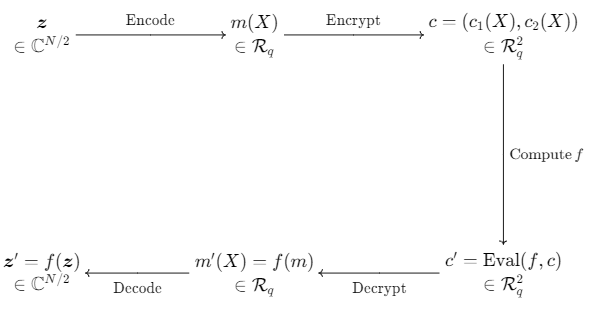
\includegraphics[]{files/figures/ckks_overview.png}
    \caption{CKKS scheme overview. Adapted \cite{openmined}}
    \label{fig:ckks_overview}
\end{figure}

HEAAN is an approximate scheme that doesn't satisfy the identity correctness property, $\dec(\sk,\enc(\pk,m))=m$. Instead, one will get $\dec(\sk,\enc(\pk,m))=m+e$, and we can guarantee that $e$ is small enough compared to $m$ so that we recover an approximate decryption of the original message. 
% https://q.uiver.app/?q=WzAsNixbMCwwLCJcXGJvbGRzeW1ib2x7en1cXFxcIFxcaW5cXG1hdGhiYiBDXntOLzJ9Il0sWzIsMCwibShYKVxcXFwgXFxpbiBcXG1hdGhjYWwgUl9xIl0sWzQsMCwiYz0oY18xKFgpLGNfMihYKSlcXFxcIFxcaW5cXG1hdGhjYWwgUl9xXjIiXSxbNCwzLCJjJz0gXFxvcGVyYXRvcm5hbWV7RXZhbH0oZixjKVxcXFwgXFxpblxcbWF0aGNhbHtSfV9xXjIiXSxbMiwzLCJtJyhYKT1mKG0pXFxcXCBcXGluIFxcbWF0aGNhbHtSfV9xIl0sWzAsMywiXFxib2xkc3ltYm9sIHonPWYoXFxib2xkc3ltYm9sIHopXFxcXCBcXGluIFxcbWF0aGJie0N9XntOLzJ9Il0sWzAsMSwiXFxvcGVyYXRvcm5hbWV7RW5jb2RlfSJdLFsxLDIsIlxcb3BlcmF0b3JuYW1le0VuY3J5cHR9Il0sWzIsMywiXFxvcGVyYXRvcm5hbWV7Q29tcHV0ZX0gZiJdLFszLDQsIlxcb3BlcmF0b3JuYW1le0RlY3J5cHR9Il0sWzQsNSwiXFxvcGVyYXRvcm5hbWV7RGVjb2RlfSJdXQ==
% \[\begin{tikzcd}
% 	{\boldsymbol{z}\\ \in\mathbb C^{N/2}} && {m(X)\\ \in \mathcal R_q} && {c=(c_1(X),c_2(X))\\ \in\mathcal R_q^2} \\
% 	\\
% 	\\
% 	{\boldsymbol z'=f(\boldsymbol z)\\ \in \mathbb{C}^{N/2}} && {m'(X)=f(m)\\ \in \mathcal{R}_q} && {c'= \operatorname{Eval}(f,c)\\ \in\mathcal{R}_q^2}
% 	\arrow["{\operatorname{Encode}}", from=1-1, to=1-3]
% 	\arrow["{\operatorname{Encrypt}}", from=1-3, to=1-5]
% 	\arrow["{\operatorname{Compute} f}", from=1-5, to=4-5]
% 	\arrow["{\operatorname{Decrypt}}", from=4-5, to=4-3]
% 	\arrow["{\operatorname{Decode}}", from=4-3, to=4-1]
% \end{tikzcd}\]

The scheme requires a process called \textit{relinearization} after each multiplication, introduced by BFV scheme \cite{bfv12} and also used in CKKS. Directly multiplying two ciphertexts $\boldsymbol c =(c_1,c_2)$ and $\boldsymbol c'=(c'_1,c'_2)$ yields a vector in $(d_0,d_1,d_2)\in \mathcal{R}_q^3$ where:
\begin{align*}
    d_0 & = c_1\cdot c'_1\\
    d_1 & = c_1\cdot c'_2 + c_2\cdot c'_1\\
    d_2 & = c_2\cdot c'_2
\end{align*}
The goal of relinearization is to transform the above triple into an equivalent tuple, i.e., a tuple that approximately preserves the decryption correctness. This process is also used in BFV and BGV schemes; although is quite expansive and introduces additional noise, it avoids ciphertext size growth, keeping it as a two-dimensional vector of polynomials.

The original HEAAN scheme was not fully homomorphic but a somewhat homomorphic one. Following Gentry's blueprint \cite{gentry2009fully}, to transform it into an FHE scheme, we should be able to evaluate the decryption circuit homomorphically, which is still an open problem for CKKS. Instead, the authors later proposed an \textit{approximate bootstrapping} procedure \cite{ckks_bootstrapping}, which follows Gentry's idea, but with an approximate decryption function. The consequence is that we lose precision after each bootstrap evaluation, but for statistical purposes, that's not a problem as long as we can control this approximation error.

\subsection{Encoding and Decoding}

The plaintext space, as we described before, is the cyclotomic ring $\Z[X]/(\Phi_M(X))$, with $M=2N$ and $N$ power of two. Our goal is to map complex $N/2$-dimensional\footnote{The reason for this dimension will soon become clearer.} vectors $\boldsymbol z\in\mathbb C^{N/2}$ into elements of the ring (encoding) and vice-versa (decoding).

We begin with the \textit{canonical embedding map}:
\begin{align*}
    \sigma &: \mathbb{C}[X]/(X^N+1)\longrightarrow\mathbb C ^N\\
    m(X)&\longrightarrow (m(\zeta_M),m(\zeta_M^3),\ldots,m(\zeta_M^{2N-1})),\\
    &\text{with }\zeta_M=\exp(2\pi i/M)
\end{align*}

The above map takes a polynomial with complex coefficients and evaluates it in the $M^{th}$ primitive roots of unity. Since $M$ is a power of two, from Definition \ref{def:prim_roots}, the primitive roots will be the $\zeta_M^k$ for $1\leq k\leq M$ with $\gcd(k, M)=1$, hence, $k$ ranges through the first $N$ odd numbers. The output is indeed a $N$- dimensional complex vector since both the polynomial coefficients and the primitive roots are complex.

An interesting fact is that $\sigma$ is an isomorphism, and we can use its inverse $\sigma^{-1}$ to encode a vector in $\boldsymbol{z}\in\mathbb C^N$ to a polynomial in $m(X)\in\C[X]/(\Phi_M(X))$. Recall that $m(X)$ can be written as $m(X)=\sum_{j=0}^{N-1}\alpha_jX^{j}$; So to construct $\sigma^{-1}$ we must be able to take $\boldsymbol z= (z_1,\ldots,z_N))^T$ and return the coefficients $(\alpha_j)_{j=0,1,\ldots,N-1}$ such that $(m(\omega_1),m(\omega_3),\ldots,m(\omega_{2N-1}))^T=\boldsymbol z$, where $\omega_k=\zeta_M^k$ to simplify notation. This can be viewed as a linear system:
\begin{align*}
    \displaystyle m(\omega_{2k-1})&=\sum_{j=0}^{N-1}\alpha_j\omega_{2k-1}^j=z_k\\
    &\text{for }k=1,2,\ldots,N;
\end{align*}
or as its matrix form:
\begin{align*}
    &~~~~~A\boldsymbol \alpha = \boldsymbol z,\\
    \text{with }A = &\left[\begin{matrix}
        1 & \omega_1 &\omega_1^2 &\ldots&\omega_1^{N-1}\\
        1 & \omega_3 &\omega_3^2 &\ldots&\omega_3^{N-1}\\
        1 & \omega_5 &\omega_5^2 &\ldots&\omega_5^{N-1}\\
        \vdots & \vdots &\vdots &\ddots&\vdots\\
        1 & \omega_{2N-1} &\omega_{2N-1}^2 &\ldots&\omega_{2N-1}^{N-1}
    \end{matrix}\right]\text{ and }\boldsymbol\alpha = \left[\begin{matrix}\alpha_0\\ \alpha_1\\ \alpha_2\\\vdots\\ \alpha_{N-1}\end{matrix}\right]
\end{align*}
The matrix $A$ is the Vandermonde matrix for the primitive roots $\omega_k=\zeta_M^k$, and has a known inverse \cite{vandermonde}. Then, we can find the coefficients through $\boldsymbol\alpha = A^{-1}\boldsymbol z$, arriving to the inverse canonical embedding map:
\begin{align*}
\sigma^{-1}:~\mathbb{C}^N&\longrightarrow\C[X]/(X^N+1)\\
    \sigma^{-1}(\boldsymbol z) &= m(X),
\end{align*}

with $m(X)=\sum_{j=0}^{N-1}\alpha_jX^j$ and $\alpha_j=(A^{-1})_j\boldsymbol z$

The complex primitive roots are symmetrical conjugates. In Figure \ref{fig:roots_of_unity} for example $\omega_1=\overline{\omega_1}=\omega_7$, in general for the $M^{th}$ primitive roots, $\omega_j=\overline{\omega_{-j}}$, where $-j$ index is taken modulo $M$. Remember that, for decoding, the goal was to map $\ring=\Z[X]/(X^N+1)$ to $\C^{N/2}$. Until now, we have a map $\ring\to\C^{N}$. The image $\sigma(\ring)$ can be reduced to half its dimension, noticing that $m(\omega_j)=\overline{m(\omega_{-j})}:$
\begin{align}
    \overline{m(\omega_{-j})}&=\overline{\sum_{k=0}^{N-1}\alpha_k\omega_{-j}^k}\nonumber
    =\sum_{k=0}^{N-1}\overline{\alpha_k\omega_{-j}^k}\nonumber\\
    &=\sum_{k=0}^{N-1}\alpha_k\overline{\omega_{-j}^k}\label{eq:real_conj}\\
    &=\sum_{k=0}^{N-1}\alpha_k\omega_{j}^k\nonumber=m(\omega_j)\nonumber
\end{align}
Equality \ref{eq:real_conj} holds because $\alpha_k\in\Z\subset\mathbb{R}$ so it does not affect the conjugate operator. Hence we have proved that the image $\sigma(\ring)$ are vectors in $\C^{N}$ whose coordinate $j$ are complex conjugates of coordinate $-j$. We can define now the subring $\mathbb{H}\subseteq \C^{N}$ as:
$$\Hr=\{(z_j)_{j\in\Z_M^*};z_j=\overline{z_{-j}},~\forall j\in \Z_M^*\},$$
where $\Z_M^*=\{k\in\Z;\gcd(k,M)=1\}=\{1,3,5,\ldots,2N-1\}$. 

The image $\sigma(\ring)$ is actually in $\Hr$. So, we can define the projection $\pi:\Hr\to\C^{N/2}$ that takes a $N$-dimensional vector in $\Hr$ and outputs a $N/2$-dimensional one, removing conjugates elements. Naturally, we also define $\pi^{-1}:\C^{N/2}\to\Hr$ that do the opposite, expanding a vector including the conjugates of its elements. Then, the decoding procedure will be $\pi\circ\sigma:\ring\to\C^{N/2}$.

Encoding is not that trivial. Notice that the codomain of $\sigma^{-1}$ is $\C[X]/(X^N+1)$, so we cannot guarantee that the polynomials will have integer coefficients. The first step is expanding $\boldsymbol z\in \C^{N/2}$ to $\Hr$ through $\pi^{-1}(\boldsymbol z)$, but to guarantee that applying $\sigma^{-1}$ will return an integer polynomial, we need to project $\pi^{-1}(\boldsymbol z)$ to the image $\sigma(\ring)$ using some rounding process $\lfloor \pi^{-1}(\boldsymbol z)\rceil_{\sigma(\ring)}$. This will approximate $\pi^{-1}$ to a close element in $\sigma(\ring)$ so that applying the inverse map results in a ring element. For more details about rounding techniques, refer to \cite{ckks17} and \cite{toolkit}. 

For precision preservation purposes, the encoding procedure multiplies $\pi^{-1}(\boldsymbol z)$ by a predefined scaling factor $\Delta>1$. Then we define $\ecd$ (encode) and $\dcd$ (decode) functions as:
\begin{align*}
    \ecd&:\C^{N/2}\longrightarrow\ring\\
    \ecd(\boldsymbol z;\Delta) &= \sigma^{-1}(\lfloor\Delta\cdot \pi^{-1}(\boldsymbol z)\rceil_{\sigma(\ring)})\\
    \dcd&:\ring\longrightarrow\C^{N/2}\\
    \dcd(m;\Delta)&=\pi\circ\sigma(\Delta^{-1}\cdot m)
\end{align*}

\subsection{Encryption, Decryption, and Relinearization}

Now let's describe the concrete cryptographic primitives of the CKKS scheme. Fix an integer base $p$ and define $q_\ell = p^{\ell}q_0$ for some given $q_0\in\Z$. This is a \textit{leveled homomorphic encryption} scheme, with levels $0\leq\ell\leq L$; after each multiplication, we rescale the message to a lower level to control the size of noise. 

The notation $\Z_q$ will choose the representatives from $\Z\cap (q/2,q/2]$, and $[ \cdot ]_q$ applied to a polynomial means wrapping its coefficients modulo $q$. $\lambda$ is a security parameter, which known attacks taking $\Omega(2^\lambda)$.

The Discrete Gaussian distribution $\dg(\sigma^2)$ over the polynomial ring $\ring$ samples the coefficients from a discrete gaussian with variance $\sigma^2$ over $\Z^N$ \cite{ckks17}; We'll use this distribution for sampling RLWE errors. Another useful distribution is $\zo(\rho)$ over $\ring_2=\Z_2[X]/(X^N+1)$, i.e., the polynomials with degree up to $N-1$ with coefficients in $\{0,\pm1\}$. $\zo(\rho)$ draws $N$ samples with probability $1-\rho$ of being zero and $\rho/2$ of being $+1$ or $-1$, this becomes the coefficients of the polynomial in $\ring_2$.

\begin{itemize}
    \item $\operatorname{KeyGen}(\lambda)$- Given a security parameter $\lambda$, chooses cyclotomical dimension $M=M(\lambda)$, error standard deviation $\sigma=\sigma(\lambda)$ and an integer $P=P(\lambda)$.
    
    Samples $s\leftarrow \ring_2$, $a\xlongleftarrow[]{\mathcal U}\mathcal{R}_{q_L}$ and $e\xlongleftarrow[]{\dg(\sigma^2)}\ring$.
    
    Set $\sk = (1,s)$ and $\pk = (b,a)$, with $b=\modulo[q_L]{-a\cdot s +e}$. Security of public key exposure is guaranteed by RLWE (Def. \ref{def:rlwe}).

    Samples $a'\xlongleftarrow[]{\mathcal U}\ring_{P\cdot q_L}$, $e'\xlongleftarrow[]{\dg(\sigma^2)}\ring$ and set the evaluation key $\evk=(b',a')$, with $b'=\modulo[P\cdot q_L]{-a'\cdot s+e'+P\cdot s^2}$. Its use will become clear soon, and security is also guaranteed by RLWE.

    \item $\enc(\pk,m)=\modulo[q_L]{v\cdot\pk+(m+e_0,e_1)},$ where $v\xlongleftarrow[]{\zo(0.5)}\ring_2$, and $e_0,e_1\xlongleftarrow[]{\dg(\sigma^2)}\ring$. Notice that the ciphertext is a two-dimensional vector of polynomials in $\ring_{q_L}$.

    \item $\dec(\sk,\boldsymbol c) = \modulo[q_\ell]{\langle\bd c,\sk\rangle}=\modulo[q_\ell]{c_1+c_2\cdot s}$, for $\boldsymbol c=(c_1,c_2)$ at level $\ell$.

    \item $\eval(+,\bd c,\bd c')=\modulo[q_\ell]{\bd c+\bd c'}$, for $\bd c,\bd c'\in\ring_{q_\ell}^2$

    \item $\eval(\evk,\times,\bd c,\bd c')=(d_0,d_1)+\lfloor P^{-1}\cdot d_2\cdot\evk\rceil(\bmod ~q_\ell)$, where for $\bd c=(c_1,c_2)$ and $\bd c'=(c'_1,c'_2)$, we have, as described before $(d_0,d_1,d_2)=(c_1\cdot c'_1,c_1\cdot c'_2 + c_2\cdot c'_1,c_2\cdot c'_2)$
\end{itemize}

The multiplication of ciphertexts is using a process called \textit{relinearizaton}, to reduce ciphertext dimension from $\ring^3_{q_\ell}$ to $\ring^2_{q_\ell}$. The goal is to find $(d_0^*,d_1^*)$ such that the decryption is approximately equivalent:
\begin{align*}
    \modulo[q_\ell]{d_0^*+d_1^*\cdot s}\approx\modulo[q_\ell]{d_0+d_1\cdot s+d_2\cdot s^2}
\end{align*}
In this case, $(d_0^*,d_1^*)=(d_0,d_1)+\lfloor P^{-1}\cdot d_2\cdot\evk\rceil(\bmod ~q_\ell)$ provides a ciphertext is an approximate valid encryption of the original multiplication of ciphertext \cite{ckks17}.

The levels $L$ define the maximum multiplicative depth the scheme allows because, after each multiplication, we rescale the ciphertext from $\ell\to\ell-1$ using:
$$\operatorname{Rescale_{\ell\to\ell'}}(\boldsymbol c) = \left\lfloor \dfrac{q_\ell'}{q_\ell}\bd c\right\rceil$$,

The intuition behind it is that each ciphertext has an embedded noise added by the encryption process, and multiplication increases it (exponentially!). the rescaling process controls the noise, reducing the ciphertext modulus together with its built-in error. For more details, refer to \cite{rescale}.

\subsection{Approximate Bootstrapping}

To make an FHE scheme out of the previously described leveled homomorphic one, we need bootstrapping, i.e., be able to evaluate the decryption function $\dec(\sk,\boldsymbol c) = \modulo[q_\ell]{\langle\bd c,\sk\rangle}$ using the homomorphic scheme. While a direct approach to homomorphically compute it is still an open problem, an \textit{approximate bootstrapping} was proposed by \cite{ckks_bootstrapping}. The idea comes from the fact that modular reduction operation can be represented by a trigonometric function:
\begin{align*}
    \modulo{\langle\bd c,\sk\rangle} = \dfrac{q}{2\pi}\cdot \sin\left(\dfrac{2\pi}{q}\cdot\langle \bd c,\sk\rangle\right) + O(\varepsilon^3\cdot q),
\end{align*} when $| \modulo{\langle\bd c,\sk\rangle}|\leq\varepsilon\cdot q$. CKKS scheme doesn't evaluate sine functions, it only permits additions and multiplications, so the authors used the Taylor expansion polynomial approximation, which can be represented as a composition of additions and multiplications.




\chapter{Private Logistic Regression}
\section{Statistical Review}
\section{Homomorphic Training}
\section{Data Applications}




